\documentclass[landscape]{article}
\usepackage[a4paper, top=0.5cm, bottom=0.5cm, left=0.5cm, right=0.5cm]{geometry}

\usepackage[utf8]{inputenc}
\usepackage{amsmath, amsfonts, amssymb}
\usepackage{multicol}
\usepackage{graphicx}
\usepackage{blindtext}
\usepackage{paralist}
\usepackage[boxed]{algorithm2e}

\setlength\parindent{0ex}
\setlength{\columnsep}{10mm}

\newcommand{\vmspace}{\vspace{-7pt}}
\newcommand{\vpspace}{\vspace{5pt}}
\newcommand{\vtspace}{\vspace{-10pt}}

\begin{document}

\pagestyle{empty}
\raggedright
\setlength{\columnsep}{2mm}
\setlength{\columnseprule}{0.1mm}
\renewcommand{\labelitemi}{--}

\begin{multicols}{3}

%\title{\textbf{Autonomous Mobile Robots}}
%\author{Fabian Bl\"ochliger}
%\date{Spring Semester 2016}
%\maketitle

\begin{tabular}{|c|}\hline
  \LARGE \textbf{Autonomous Mobile Robots}\\[6pt]
  \large Fabian Bl\"ochliger\\[6pt]
  \large \textit{Spring Semester 2016}\\\hline
\end{tabular}

\vtspace

\section{Introduction and Motivation}

\vmspace

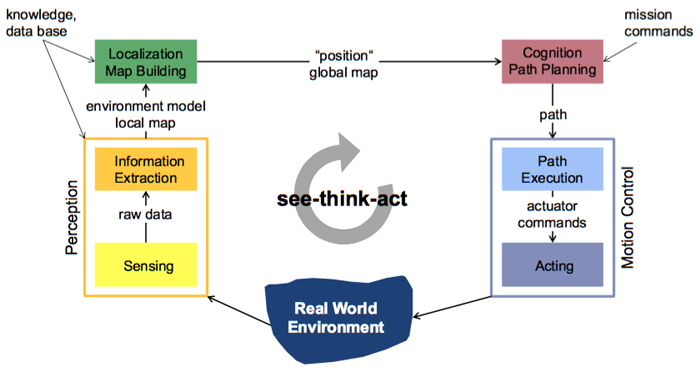
\includegraphics[width=\columnwidth]{img/1_SeeThinkAct.png}

\vspace{-12pt}

\section{Locomotion Concepts}

\vmspace

\begin{minipage}{\columnwidth}
  To get from the inertial frame $I$ to body frame $B$:
  \begin{compactitem}
    \item \textbf{translate} with vector ${}_I\mathbf{r}_{OB}$,
    \item \textbf{rotate} with matrix $\mathbf{R}_{IB}$.
  \end{compactitem}
\end{minipage}

\vpspace

\begin{minipage}{\columnwidth}
  Express point $P$ which is given w.r.t frame $B$ in frame $I$:
  \vmspace
  \begin{center}
  ${}_I\mathbf{r}_{OP} = {}_I\mathbf{r}_{OB} +
  \mathbf{R}_{IB}\;{}_B\mathbf{r}_{BP}$.
  \end{center}
\end{minipage}

\vpspace

\begin{minipage}{\columnwidth}
  Equivalent \textbf{homogeneous transformation} description:
  \vmspace
  \begin{center}
    $\left(\begin{matrix}
      {}_I\mathbf{r}_{OP} \\
      1
    \end{matrix}\right)
    =
    \left(\begin{matrix}
      \mathbf{R}_{IB} & {}_I\mathbf{r}_{OB} \\
      0 & 1
    \end{matrix}\right)
    \left(\begin{matrix}
      {}_B\mathbf{r}_{BP} \\
      1
    \end{matrix}\right)$
  \end{center}
\end{minipage}

\vpspace

\begin{minipage}{\columnwidth}
  \textbf{Velocity} of rigid body point $P$:
  \vmspace
  \begin{center}
    ${}_I \mathbf v_P = {}_I \mathbf{\dot r}_{OP} = \mathbf{\dot r}_{OB} +
    {}_I\mathbf{\omega}_{IB} \times {}_I\mathbf r_{BP}.$
  \end{center}
\end{minipage}

\vpspace

\begin{minipage}{\columnwidth}
  \textbf{Differentiation} of moving frame vector:
  \vmspace
  \begin{center}
    ${}_B\mathbf v_P = {}_B\left(\mathbf{\dot r}_{OP}\right) = \dfrac{\mathrm
    d\, {}_B\mathbf r_{OP}}{\mathrm d \,t} + {}_B\omega_{IB} \times {}_B\mathbf
    r_{OP}$
  \end{center}
\end{minipage}

\vpspace

\begin{minipage}{\columnwidth}
  Basic rotation matrices $\mathbf R_x(\bullet)$, $\mathbf R_y(\bullet)$, $\mathbf
  R_z(\bullet)$:
  \vmspace
  \begin{center}
    $\left(\begin{matrix}
      1 & 0 & 0 \\
      0 & \cos & -\sin \\
      0 & \sin & \cos
    \end{matrix}\right),\;
    \left(\begin{matrix}
      \cos & 0 & \sin \\
      0 & 1 & 0 \\
      -\sin & 0 & \cos
    \end{matrix}\right),\;
    \left(\begin{matrix}
      \cos & -\sin & 0 \\
      \sin & \cos & 0 \\
      0 & 0 & 1
    \end{matrix}\right).$
  \end{center}
\end{minipage}

\vpspace

\begin{minipage}{\columnwidth}
  \textbf{Jacobian} (partial derivative of position vector $\mathbf{r}_{OP}$
  w.r.t. \textbf{generalized coordinate} vector $\mathbf{q}$):
  \vmspace
  \begin{center}
    $J_P = \dfrac{\partial \mathbf{r}_{OP}(\mathbf q)}{\partial \mathbf q}$.
  \end{center}
\end{minipage}

\vpspace

\begin{minipage}{\columnwidth}
  Left/right pseudoinverse for $m \times n$ matrix $\mathbf{J}$ to solve
  $\mathbf r_F = \mathbf J_F \mathbf q$ for $\mathbf q$:
  \vmspace
  \begin{center}
    $\mathbf{J}^+=
    \begin{cases}
      (\mathbf{J}^\intercal \mathbf J)^{-1} \mathbf J^\intercal, & m>n\;\;
      \text{(overdetermined)},\\
      \mathbf J^\intercal (\mathbf{J} \mathbf J^\intercal)^{-1}, & m<n\;\;
      \text{(underdetermined).}
    \end{cases}$
  \end{center}
\end{minipage}

\vpspace

\begin{minipage}{\columnwidth}
  Iterative approach for \textbf{inverse kinematics} of robotic manipulator to
  find generalized coordinates for end-effector position $\mathbf r^\text{goal}$
  (Newton's method):\\
  \vmspace
  \begin{algorithm}[H]
    $\mathbf q = \mathbf q^0,\;\mathbf r = \mathbf r(\mathbf q)$\;
    \While{$\| \mathbf r - \mathbf r^\mathrm{goal} \| > \mathrm{threshold}$}
    {
    $\mathbf q = \mathbf q + \mathbf J^+(\mathbf q) \cdot (\mathbf r^\text{goal}
    - \mathbf r),\;\;
    \mathbf r = \mathbf r ( \mathbf q )$\;
    }
  \end{algorithm}
\end{minipage}

\vpspace

\begin{minipage}{\columnwidth}
  Inverse \textbf{differential kinematics} (get desired end-effector velocity
  $\mathbf{\dot{r}_F}$):
  \vmspace
  \begin{center}
    $\mathbf{\dot r}_F = \mathbf J_F \mathbf{\dot q}$
    $\;\;\rightarrow\;\;$
    $\mathbf{\dot q} = \mathbf J_F^+ \mathbf r_F.$
  \end{center}
\end{minipage}

% TODO
% - Check column-rank / row-rank deficiency.

\vtspace

\section{Mobile Robot Kinematics}

\vmspace

\begin{minipage}{\columnwidth}
\textbf{Fixed/steered standard wheel} model with robot frame $R$, steering frame
$S$ and wheel frame $W$:
\vmspace
\vmspace
\begin{center}
  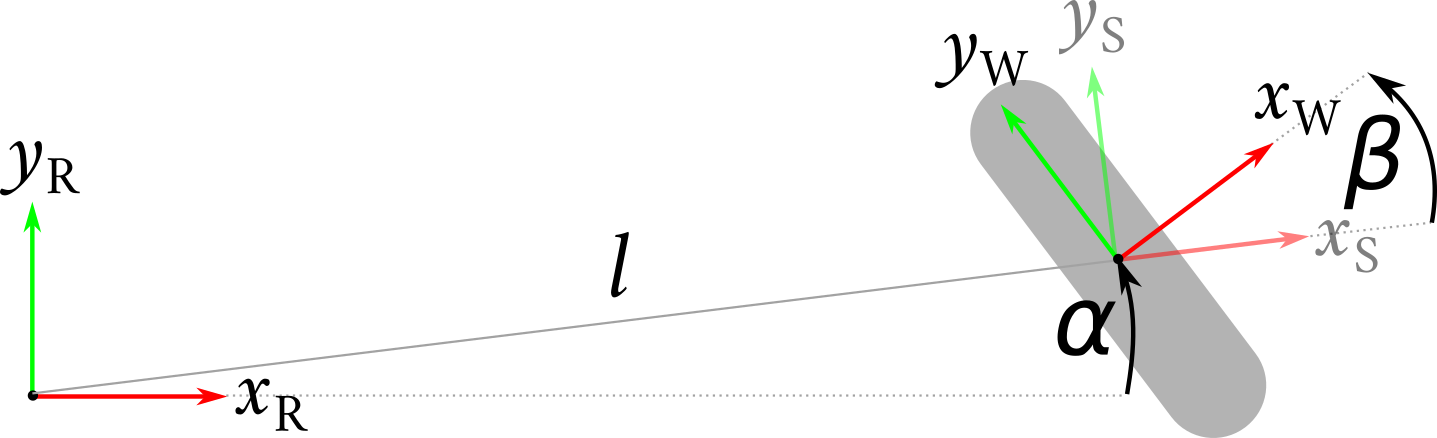
\includegraphics[width=0.9\columnwidth]{img/3_Wheel.png}
\end{center}
\end{minipage}


\begin{minipage}{\columnwidth}
  Rolling constraint:
  \vmspace
  \begin{center}
    $\left[\begin{matrix}
      \sin(\alpha + \beta) & -\cos(\alpha + \beta) & (-l) \cos(\beta)
    \end{matrix}\right]
    R(\theta)\dot\xi_I
    =
    r \dot \varphi.$
  \end{center}
\end{minipage}

\begin{minipage}{\columnwidth}
  No-sliding constraint:
  \vmspace
  \begin{center}
    $\left[\begin{matrix}
      \cos(\alpha + \beta) & \sin(\alpha + \beta) & l \sin(\beta)
    \end{matrix}\right]
    R(\theta)\dot\xi_I
    =
    0.$
  \end{center}
\end{minipage}

\begin{minipage}{\columnwidth}
  Robot state:
    $\xi_I
    =
    \left[\begin{matrix}
      x & y & \theta
    \end{matrix}\right]^\intercal,
    \;\;
    \dot\xi_R = R(\theta)\dot\xi_I,
    \;\;
    R(\theta) = \mathbf R_z^\intercal(\theta).$
\end{minipage}

\vpspace

\begin{minipage}{\columnwidth}
  Stacked equations of motion for a $(N_f+N_s)$-wheeled robot:
  \vmspace
  \begin{center}
    $\begin{matrix}
      \text{\textbf{(rolling)}}\;\;\;\;\;\; \\
      \text{\textbf{(no-sliding)}}
    \end{matrix}\;\;
    \left[\begin{matrix}
      J_1(\beta_s) \\
      C_1(\beta_s)
    \end{matrix}\right]
    R(\theta)\dot\xi_I
    =
    \left[\begin{matrix}
      J_2 \\
      0
    \end{matrix}\right]
    \dot\varphi,\;\;\;\;
    \dot\varphi
    =
    \left[\begin{matrix}
      \varphi_1..\varphi_N
    \end{matrix}\right],$
  \end{center}
\end{minipage}

\begin{minipage}{\columnwidth}
  with
  \vmspace
  \begin{center}
    $J_1(\beta_s)
    =
    \left[\begin{matrix}
      J_{1f} \\
      J_{1s}(\beta_s)
    \end{matrix}\right],
    J_2
    =
    \mathrm{diag}(r_1..r_N),
    C_1(\beta_s)
    =
    \left[\begin{matrix}
      C_{1f} \\
      C_{1s}(\beta_s)
    \end{matrix}\right].$
  \end{center}
\end{minipage}

\vpspace

\begin{minipage}{\columnwidth}
  A robot's \textbf{degree of maneuverability} $\varphi_M$ is
  \vmspace
  \begin{center}
    $\delta_M = \delta_m + \delta_s$,
  \end{center}
  \vmspace
  which is the sum of its \textbf{degree of mobility} $\varphi_m$ and its
  \textbf{degree of steerability} $\varphi_s$:
  \vmspace
  \begin{center}
    $\delta_m=\mathrm{dim}\,\mathrm{N}\left[C_1(\beta_s)\right] = 3 -
    \mathrm{rank}\left[C_1(\beta_s)\right],\;
    \varphi_s = \mathrm{rank}\left[C_{1s}(\beta_s)\right].$
  \end{center}
\end{minipage}

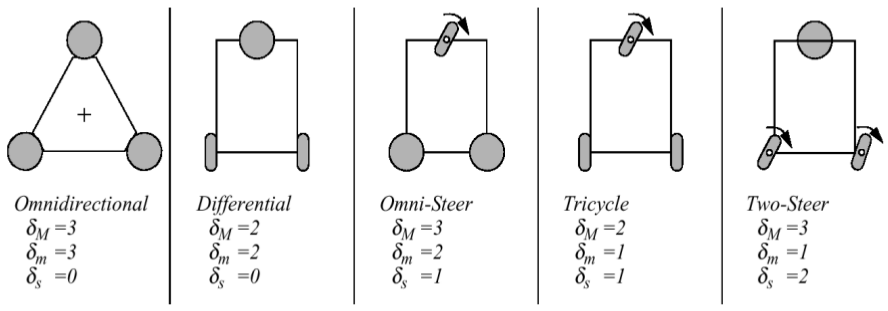
\includegraphics[width=\columnwidth]{img/3_WheelTypes.png}

\vmspace

(Two robots with the same $\varphi_M$ may not be equivalent
\textbf{instantaneously}.)

\vtspace

% TODO
% Add if more space:
% - differential kinematics

\section{Perception I}

\blindtext[3]

\section{Perception II}

\blindtext[3]

\section{Perception III}

\blindtext[3]

\section{Perception IV}

\blindtext[3]

\section{Localization I}

\blindtext[3]

\section{Localization II}

\blindtext[3]

\section{SLAM I}

\blindtext[3]

\section{SLAM II}

\blindtext[3]

\section{Planning I}

\blindtext[3]

\section{Planning II}

\blindtext[3]





\end{multicols}

\end{document}
